\documentclass[a4paper]{article}

\usepackage{microtype}
\usepackage{fullpage}
\usepackage{amsmath}
\usepackage{hyperref}
\usepackage{graphicx}
\usepackage{amsthm}
\usepackage{amssymb} 
\usepackage{booktabs}
\usepackage[labelsep=period]{caption}
\usepackage{subcaption}
\usepackage[noabbrev,nameinlink]{cleveref}
\usepackage[section]{placeins}
\usepackage{listings}
\usepackage{setspace}
\usepackage{snapshot}
\usepackage{apptools}
\usepackage[backend=biber,style=authoryear,maxbibnames=99,hyperref=true]{biblatex}
\usepackage{mfirstuc}

\setstretch{1.15}

\hypersetup{colorlinks, citecolor=blue, filecolor=blue, linkcolor=blue, urlcolor=blue}

\addbibresource{src/paper/references.bib}
\DeclareFieldFormat{jtnoformat}{\capitalisewords{#1}}

\newcommand*{\latestversion}{\normalsize{Latest version: \href{https://stanmart.github.io/phd-thesis/experiment.pdf}{stanmart.github.io/phd-thesis/experiment.pdf}}}

\DeclareMathOperator*{\argmax}{argmax}

\newtheorem{proposition}{Proposition}

\AtAppendix{\counterwithin{proposition}{section}}
\AtAppendix{\counterwithin{equation}{section}}
\AtAppendix{\counterwithin{figure}{section}}
\AtAppendix{\counterwithin{table}{section}}

\lstset{
    basicstyle=\footnotesize\ttfamily,
    columns=flexible,
    breaklines=true,
}


\title{
    Characterizing Multiplayer Free-Form Bargaining: A Lab experiment%
    \thanks{
        We would like to thank our advisors, Nick Netzer, Marek Pycia, Armin Schmutzler, and Jakub Steiner for their invaluable feedback and support throughout this project.
        We are also grateful to Sandro Ambühl and Roberto A. Weber for the thoughtful suggestions about the design of the experiment.
        Finally, we thank the participants of the Behavioral Lab Meetings and the Market Design Seminar for their questions and comments.
    }
}

\author{
    Mia Lu\thanks{University of Zurich, mia.lu@econ.uzh.ch} 
    \and 
    Martin Stancsics\thanks{University of Zurich, martin.stancsics@econ.uzh.ch}
}

\date{July 30, 2024 \\ \latestversion} 

\begin{document}

\maketitle

\section{Motivation}

Although market structures resembling various aspects of what we call platforms have existed for some time, the term has only gained widespread usage in the 2000s, with the advent of digitization, and a number of behemoth technology companies playing matchmakers on the internet.
Since then, platforms have become a buzzword in the business world, the subject of increasing regulatory scrutiny, and also a topic of intense academic interest.
Platforms have a number of unique features that make them different from more traditional market structures.
The most prominent of those are multi-sidedness and network effects, which most of the early literature \parencite[for an overview, see][]{rochet2006two} and policy debate \parencite[e.g.][]{fletcher2021consumer,calvano2021market} has focused on.
However, in the more recent years, another important and potentially concerning aspect has been getting more attention: the hybrid operation of certain platforms.
Essentially, this means that platforms act as an intermediary (deciding the rules) and a market participant (competing with other entrants) at the same time.

While hybrid platforms are not a completely new phenomenon, they are becoming more and more common in various industries.
Perhaps the most prominent example is Amazon, which, on the one hand sells its own products, and at the same time hosts ax large number of third-party sellers.
However, examples abound in other industries, as well.
For example, each of the largest digital distribution platforms for computer and smartphone applications (Google Play, Apple App Store and Microsoft Store) sell their own applications besides their third party offerings.
In the video game industry, platform owners studios and publishing games under their own brand is the standard.
Many video streaming services (e.g. Netflix, Amazon Prime Video, Hulu) offer a mix of their own and licensed content.
One can also find examples of similar behavior outside the platform setting, too.
For example, a number of car manufacturers are planning to sell directly to consumers in addition to selling through their dealership networks.

As deciding the rules of the game and competing in it at the same time gives rise to some obvious concerns, policymakers have been paying increasingly close attention to these platforms in the recent years.
Various pieces of legislation have been proposed to regulate, or even ban e-commerce platforms from selling their own products \parencite[][]{phartiyal_2019,reynolds_2022,eu-2022}.
Furthermore, one of the most prominent recent antitrust cases, Microsoft acquiring the video game publisher Activision/Blizzard for a sum of 69 billion USD, is also a case of a platform becoming increasingly hybrid.
This merger not only increased market concentration on the software side of the video game industry, but might also have further implications for the competition between Microsoft as a platform owner and the other game developers.
The deal was under investigation by multiple antitrust authorities, including the US Federal Trade Commission, the European Commission, and the UK Competition and Markets Authority \parencite{livni_merced_2023}.

In parallel to the increasing regulatory interest, the academic literature on the topic of hybrid platforms has also been steadily growing.
\textcite{hagiu2022should} investigate how practices, such as self-preferencing and steering can distort competition on hybrid platforms.
They argue that -- while such practices are problematic and can have negative welfare effects -- with proper regulation the platform selling its own products can be beneficial for consumers.
In contrast to this positive result, \textcite[]{anderson2021hybrid} find that even in the absence of such behavior, allowing hybrid operation might have negative consequences due to platforms having an incentive to exclude competitors from the market.
\textcite[]{gutierrez2021welfare} shows that general conclusions are hard to draw, and welfare effects are platform and product specific.
For example, using a mechanism design approach, \textcite{kang2022contracting} demonstrate that welfare consequences greatly depend on whether the platform faces competition in the upstream market.

This paper aims to contribute to this discussion by examining an important, but so far underexplored aspect of platforms: the bargaining power disparity between them and the other market participants, and how this disparity is affected by the platforms' hybrid operation.
I propose an analytically tractable model of a which captures many important aspects of bargaining between one large and a continuum of small players: namely a hybrid platform facing a continuum of potential entrants.
I show that, in the presence of bargaining, hybrid operation can indeed have negative welfare consequences for consumers.
This result is particularly striking in this otherwise distortion-free\footnote{
    In the benchmark model without bargaining, the platform's hybrid operation does not affect consumer welfare.
} setting. 
The intuition is that hybrid operation increases the platform's bargaining power against the entrant sellers.
This in turn leads to a higher entry fee, fewer entrants, then results in lower consumer surplus.
These observations constitute a so-far overlooked aspect of hybrid platforms that policymakers should be aware of.
Due to the relative generality of this model, these results are applicable not only to hybrid platform, but to other similar settings, such as upstream producers having their own downstream outlets, or retailers with private labels, as well.

Many of the results are not tied to the specifics of the model, but are more general instead.
They do not depend on a specific demand structure and investment cost assumptions, and there is even some flexibility to the assumptions about bargaining outcomes.
I show that, even in such stylized setting, some interesting observations can be made about the effects of hybrid operation. 
In particular, when the platform's and the potential entrants' products are substitutes, increasing the platform's product variety will lead to a decrease in the number of entrants.
I also give sufficient conditions for this decrease in entry being so large as to cause a decrease in total profits, as well.

The closest model to the one proposed in this paper is \textcite{anderson2021hybrid}.
The key difference between the two boils down to how the entry fee is decided.
In \textcite{anderson2021hybrid}, the platform sets a percentage entry fee, and the entrants decide whether to enter or not.
In contrast to this, I assume that (1) platforms charge a lump-sum entry fee and that (2) this entry fee is the result of a negotiation process\footnote{
    The bargaining process is modeled using a solution concept from cooperative game theory, namely the Shapley-value.
    This allows for a tractable analysis while at the same time capturing many of the important features of bargaining.
    Examples of this approach in the industrial organization literature include \textcite{montez2007downstream}, as well as \textcite{hart1990property}, \textcite{levy1997individual}, \textcite{inderst2003bargaining} and \textcite{brugemann2019intra} among others.
}
between the platform and the entrants.
The second point is a novelty not only compared to \textcite{anderson2021hybrid}, but also to the existing literature on hybrid platforms.
Furthermore, in contrast to \textcite{hagiu2022should}, this model is free from any distortive behavior, such as self-preferencing or steering, and the negative results are purely driven by changes in the platform's bargaining position.

The set of more general results in this paper go beyond the aforementioned studies in the sense that they illuminate the effects of hybridness as a more abstract phenomenon, and thus also highlight the similarities between the hybrid platform literature and adjacent ones.
Certain structures, such as vertical relationships, or even traditional retail stores share a number of features with platforms (notably, the presence of a dominant, indispensable entity), and can be modeled in much the same way.
Therefore, the methodology and results in this paper are also of interest to researchers studying questions such as retailers having their own private labels \parencite{steiner2004nature} or vertical integration in upstream-downstream markets \parencite{hart1990vertical,aghion2006vertical}.
\textcite{de2005vertical} and \textcite{montez2007downstream}, in which bargaining between the upstream and downstream firms take the center stage, are particularly closely related.
Among empirical studies in related settings, \textcite{ho2017insurer} looks at the effect of insurer competition on health care prices, while \textcite{crawford2018welfare} explores the effects of vertical integration on television markets.

This paper is also related to various other strands of the industrial organization literature.
Most generally, it is a contribution to the research agenda on understanding platforms and their role in the economy \parencite[e.g.][]{rochet2003platform,hagiu2004optimal,armstrong2006competition,evans2011platform,lee2014competing}.
Furthermore, it is somewhat adjacent to the literature on the importance of exclusive content \parencite[e.g.][]{hagiu2011exclusivity,lee2013vertical,dou2014sell,weeds2016tv}, with the difference that instead of exclusive content giving an advantage against competing platforms, in this paper, own products provide an advantage over potential entrants.
More generally, many results and concepts of this paper are also applicable outside the context of (multi-sided) platforms.

Finally, this paper also belongs to the not too large set of models using concepts from cooperative game theory in an industrial organization setting.
Such examples include the aforementioned \textcite{montez2007downstream}, as well as \textcite{hart1990property}, \textcite{levy1997individual}, \textcite{inderst2003bargaining} and \textcite{brugemann2019intra}, among others.
In contrast to the majority of those, which focus on games with a finite number of players, I utilize an oceanic game (a continuum of small players instead of a finite number), and demonstrate that this can considerably simplify the analysis in certain cases.
Therefore, the modeling approach presented in this paper may be of use in other settings as well.

The rest of the paper is organized as follows.
In \Cref{sec:model}, I introduce two model of hybrid platforms: a benchmark with the platform setting an entry fee unilaterally, and the main model, where the platform and the fringe firms engage in bargaining.
After that, \Cref{sec:results} demonstrates that the two have very different implications for consumer welfare.
\Cref{sec:extensions} then examines the effect of different assumptions about the bargaining process.
Finally, \Cref{sec:conclusion} summarizes the results and discusses possible future work.


\section{Model}
\label{sec:model}

This section introduces the model used throughout the paper.
% TODO: better motivation
I use the terms ``platform'' and ``fringe sellers'', and present my ideas in the context of an intermediated market, such as an online marketplace or an application store.
However, the model is quite general, and the results apply to a broader class of settings, such as vertical markets where the upstream firm can sell directly to consumers, or retail stores with their own private labels.
Furthermore, while the discussion in the main text focuses on a specific demand structure and profit sharing rule, most of the results apply to a broader class of models.
\Cref{sec:more_general} explores the generalizability of these results, and highlights some common themes in settings with hybrid behavior.

Assume that there are two types of players in the market: a platform $P$, a continuum of fringe sellers $F_i$ ($i \in \mathbb{R}^+$) and a continuum of consumers $C_j$ ($j \in [0, 1]$).
The fringe firms have one product each, which they can only sell through the platform.
Without the platform, they make zero profits.
In addition to acting as an intermediary between the fringe and the consumers, the platform itself may also produce and sell a number of products directly to the consumers.
If it does, it is referred to as a hybrid platform.

The main distinguishing feature of this model is that, instead of assuming that entry fees or royalties are set by the platform and the fringe treat it as take it or leave it offers, I assume that the platform and the fringe engage in some kind of bargaining over their total profits.
The bargaining rule, as well as other details of the model, are described in the rest of this section.

The rest of this section is structured as follows.
\Cref{sec:model_overview} provides an overview of the model's stages, the timing of the game, as well as the qeuilibrium concept used in this paper.
Then, \Cref{sec:model_details} describes each stage of the game formally.
Finally, \Cref{sec:model_discussion} discusses some of the assumptions made in the model, and their implications.

\subsection{Overview and timing}
\label{sec:model_overview}

I consider two versions of the model: a benchmark case with the platform setting the entry fee unilaterally, and a bargaining model where the platform and the fringe firms negotiate over the entry fee.
Each version has four main stages corresponding to determining four sets of endogenous variables: (1) the platform (and the fringe) setting (negotiating) the entry fee, (2) the fringe firms deciding whether to enter the market, (3) the platform and the fringe setting the prices of their products, and (4) consumers making their purchase decisions.
The main difference between them lies in how the entry fee is determined, and, correspondingly, the order of the first two stages.

The timing of both models is illustrated in \Cref{fig:timing}.
The square brackets indicate the endogenous variables decided at that stage of the game.
In the benchmark model (\Cref{fig:timing_benchmark}), the game starts by the platform announcing and committing to an entry fee $K_F$ ($\mathbf{T_1}$).
Next, each fringe firm decides whether to create a product at cost $I_F$ and enter the market. ($\mathbf{T_2}$)
After that, the platform and the fringe firms simultaneously choose the prices for their products, engaging in monopolistic competition ($\mathbf{T_3}$).
Finally, consumers make their purchase decisions, and profits are realized ($\mathbf{T_3}$).

The bargaining model has a slightly different timing, as shown in \Cref{fig:timing_bargaining}.
The platform cannot commit to an entry fee at the beginning, so the game starts with the fringe firms deciding whether to invest in creating a product at cost $I_F$ ($\mathbf{T_1}$).
After that, the entry fee is decided as a result of some negotiation\footnote{
    The negotiation process, or rather its outcome is described in detail in \Cref{sec:cooperative_game}.
} between the platform and the firms that have made the investment ($\mathbf{T_2}$).
Then, the firms that made the investment pay the platform entry fees, too.
From this point on, the game proceeds in the same way as in the benchmark model: the platform and the fringe firms set their prices ($\mathbf{T_3}$), and consumers make their purchase decisions ($\mathbf{T_4}$). 

The main difference between the benchmark and the bargaining model is in determining the entry fee $K_F$.
In the former, the platform unilaterally sets the fee, and the fringe treats it as a take it or leave it offer.
On the other hand, in the bargaining model, I assume that the entry fee is the result of a negotiation between the parties.
More precisely, in the latter case, I assume that the platform's and the fringe's total profits at the end of the game correspond to their Shapley values.
This in turn uniquely determines the entry fee, and thus the negotiation at time ($\mathbf{T_2}$) can be equivalently conceptualized as bargaining over the final profit as well as the entry fee.

\begin{figure}
    \centering
    \begin{subfigure}{0.45\textwidth}
        \centering
        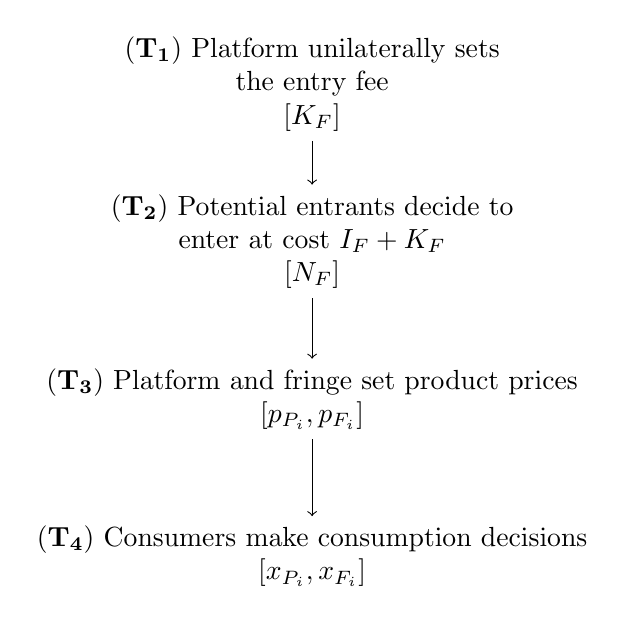
\begin{tikzpicture}[node distance=2cm, auto]
            \node[align=center] (entry_fee) {($\mathbf{T_1}$) Platform unilaterally sets \\ the entry fee \\ $[K_F]$};
            \node[align=center] (entry_decision) [below of=entry_fee] {($\mathbf{T_2}$) Potential entrants decide to \\ enter at cost $I_F + K_F$ \\ $[N_F]$};
            \node[align=center] (sales) [below of=entry_decision] {($\mathbf{T_3}$) Platform and fringe set product prices \\ $[p_{P_i}, p_{F_i}]$};
            \node[align=center] (final) [below of=sales] {($\mathbf{T_4}$) Consumers make consumption decisions \\ $[x_{P_i}, x_{F_i}]$};
            \draw[->] (entry_fee) -- (entry_decision);
            \draw[->] (entry_decision) -- (sales);
            \draw[->] (sales) -- (final);
        \end{tikzpicture}
        \caption{Benchmark model (platform sets the entry fee unilaterally)}
        \label{fig:timing_benchmark}
    \end{subfigure}
    \hfill
    \begin{subfigure}{0.45\textwidth}
        \centering
        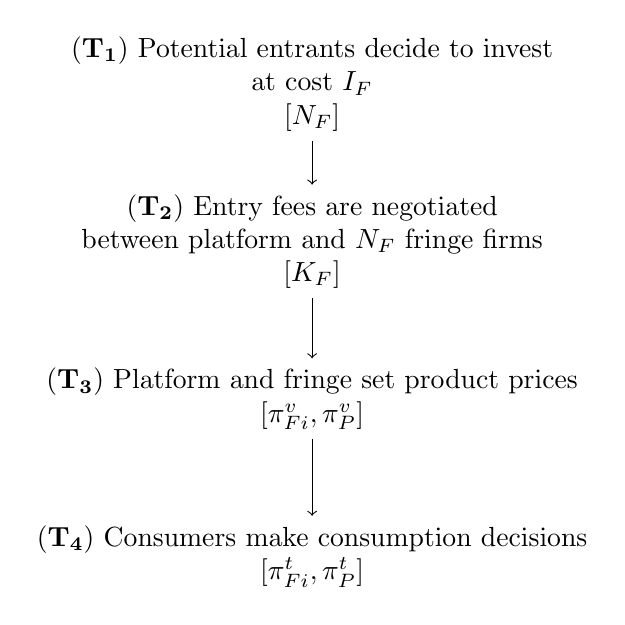
\begin{tikzpicture}[node distance=2cm, auto]
            \node[align=center] (entry_decision) {($\mathbf{T_1}$) Potential entrants decide to invest \\ at cost $I_F$ \\ $[N_F]$};
            \node[align=center] (entry_fee) [below of=entry_decision] {($\mathbf{T_2}$) Entry fees are negotiated \\ between platform and $N_F$ fringe firms \\ $[K_F]$};
            \node[align=center] (sales) [below of=entry_fee] {($\mathbf{T_3}$) Platform and fringe set product prices \\ $[\pi_{Fi}^v, \pi_P^v]$};
            \node[align=center] (final) [below of=sales] {($\mathbf{T_4}$) Consumers make consumption decisions \\ $[\pi_{Fi}^t, \pi_P^t]$};
            \draw[->] (entry_decision) -- (entry_fee);
            \draw[->] (entry_fee) -- (sales);
            \draw[->] (sales) -- (final);
        \end{tikzpicture}
        \caption{Bargaining model (platform and fringe negotiate over the entry fee)}
        \label{fig:timing_bargaining}
    \end{subfigure}
    \caption{Timing of the models}
    \label{fig:timing}
\end{figure}

For both models, this structure corresponds to a perfect-information extensive-form game.
As a consequence, the solution concept I use is the subgame perfect equilibrium.
As the platform's product variety ($N_P$) is assumed to be exogenous, the only strategic variables are (1) the fringe players' entry decisions, (2) the platform's entry fee (only in the benchmark model), (3) the prices of the products and (4) the consumers' purchase decisions.

In these two specific games, the subgame perfect can be charactrerized as follows.
\begin{definition}
    \label{def:equilibrium}
    An equilibrium of the game is a tuple $(N_F, K_F, p_{P_i}, p_{F_i}, x_{P_i}, x_{F_i})$ such that:
    \begin{enumerate}
        \item The fringe entrants make zero total profits (including the investment cost $I_F$ and the entry fee $K_F$).
        \item The platform's entry fee $K_F$ is such that
        \begin{description}
            \item[benchmark case:] they maximize total platform profits;
            \item[bargaining case:] total platform profits are equal to the Shapley value of the platform.
        \end{description}
        \item Product prices $p_{F_i}$ and $p_{P_i}$ are such that they maximize per-product profits, given the products on the market ($P_i, i \in [0, N_P]$ and $F_i, i \in [0, N_F]$).
        \item $x_{F_i}$ and $x_{P_i}$ are the outcome of consumers maximizing their utility, given the prices.
    \end{enumerate}
\end{definition}

\subsection{Details}
\label{sec:model_details}

\subsubsection{Demand}
\label{sec:demand}

Let us now describe each stage of the game in more detail, starting with the final two subgames, as they are identical in both models.
This part of the model is based on \textcite[]{anderson2021hybrid}, who utilize the exact same utility structure as th one described here.
Imagine that there is a unit mass of consumers, looking to buy one product each.
They choose from a continuum of products, which are either produced by the fringe (indexed by $F_i$), by the platform ($P_i$) and a unit mass of outside options ($0_i$).
Customer $j$ derives the following utility from buying product $T_i$\footnote{
    To avoid duplication, I denote the different types of products by $T_i$, where $T \in \{F, P, 0\}$ (fringe products, platform profucts, and outside options, respectively).
    This notation is used throughout the paper for other variables having fringe and platform counterparts, as well.
}:
\begin{align*}
    u_{T_i}^j = v_{T_i} - p_{T_i} + \mu\epsilon_{T_i}^j \quad \text{for } T_i \in \{F, P\},
\end{align*}
where $v_{T_i}$ is the value of product $T_i$, $p_{T_i}$ is its price, and $\epsilon_{T_i}^j$ is an idiosyncratic taste shock.
Throughout this section I assume that the value of each fringe product is the same, and the same goes for the platform products.
I.e., $v_{T_i} = v_T \, \forall\,i$.
This is to simplify the analysis, but is not crucial for the results.

$\epsilon_{T_i}^j$ is assumed to be independent and identically distributed (i.i.d.) across consumers and products, and follow a standardized Type I Extreme Value distribution.
This distributional assumption, along with the fact that each consumer consumes only one product, will lead to a tractable, logit-form demand function.
The demand for product $T_i$ is that arises from the consumers maximizing their utility is denoted by $x_{T_i}$.

\subsubsection{Production}

Each (horizontally differentiated) product is produced by a single, monopolistically competitive (fringe) seller.
The production entails a constant marginal cost $c_{T_i}$.
As with the value, I assume that the marginal cost is the same for all products: $c_{T_i} = c_T$.
Facing the demand described in the previous paragraphs, the sellers choose their price $p_{T_i}$ to maximize profits.
The price of the outside option is normalized to zero.

\subsubsection{Fringe entry and platform fees}

Now let us turn to stage 1 and 2 of the game: the determination of the entry fee and the fringe firms' entry decision.
I start with the benchmark model, where the platform sets the entry fee unilaterally.
Then, I compare and contrast this with the bargaining model, where the entry fee is the result of a negotiation between the platform and the fringe firms.

\paragraph{Benchmark case}

I assume that there is a continuum of potential fringe entrants, indexed by $i \in \mathbb{R}^+_0$.
Each of them can create a product at an exogenous investment cost $I_F$.
If they decide not to, they make zero profits and do not participate in the later stages of the game.
Furthermore, these firms can only sell their products through the platform, for which the platform can charge a lump-sum entry fee $K_F$.
The timing of these decisions is as follows: (1) the platform sets and commits to an entry fee $K_F$, (2) the fringe firms decide whether to enter the market and pay investment cost $I_F$ and entry fee $K_F$.

\paragraph{Bargaining case}
\label{sec:model_bargaining}

In contrast to the benchmark model, in this case, the platform cannot commit to an entry fee: it is decided as a result of a negotiation between the platform and the fringe firms.
In order to keep the model tractable, I model this in a reduced-form manner: I assume that the platform and the entrants agree on an entry fee $K_F$, which makes the total profits net entry fees equal to the Shapley value of the players.
Due to this assumption, the timing of the model is also different.
First, the fringe firms decide whether to invest in creating a product at cost $I_F$.
After this, the platform and the firms that have made the investment negotiate the entry fee.
Finally, the firms that have entered pay the entry fee to the platform.

More specifically, the resulting entry fees look as follows.
Assume that $N_F$ fringe firms choose to invest in creating a product in the first stage of the game.
Now, for every $s N_F$ ($s \in [0, 1]$), calculate the total profits that would be realized if the platform and $n_f$ fringe firms were the only players in the market, and they engaged in monopolistic competition as described in the previous paragraph.
Let us denote these profits by $\pi^v_{F}(N_P,s N_F)$ and $\pi^v_{P}(N_P,s N_F)$, and the corresponding industry-wide total profits by $\Pi$ and $\Pi(N_P,s N_F)$.\footnote{
    Throughout this paper, I use the notation $\pi_T$ to denote the profits realized by player(s) $T$, and $\Pi$ to denote the total industry profits.
    Furthermore, $\pi^v_T$ denotes profits from sales (i.e., profits not including investment costs and entry fees), whereas $\pi^t_T$ stands for total profits.
}

\begin{proposition}
    \label{prop:shapley_value}
    The Shapley value of the platform and the fringe firms, and thus final total profits, are given by:
    \begin{align*}
        \pi^t_P(N_P, N_F) &= \int_0^1 \Pi(N_P,s N_F) \ds, \\
        \pi^t_F(N_P, N_F) &= \int_0^1 \partial_2 N_F \Pi(N_P,s N_F) \ds.
    \end{align*}
\end{proposition}
\begin{proof}[Proof of \Cref{prop:shapley_value}]
    The cooperative game is describer in detail in \Cref{sec:cooperative_game_one_sided}.
    This result is a direct consequence of \Cref{prop:profit_sharing_one_sided}.
\end{proof}

\subsection{Discussion}
\label{sec:model_discussion}

Let us now discuss some of the non-standard assumptions made in the model, and their implications.
I look at four main categories in this section: the timing of the game, the costs of entry for fringe firms, the way the monopolistic competition is modeled, and the way the bargaining process is modeled.

\subsubsection{Costs of entry}

For each potential fringe entrant $F_i$, entering the marker has two, separate costs: an exogenous investment cost $I_F$, and the lump-sum platform entry fee $K_F$.
One can conceptualize the first one, $I_F$, as usual fixed costs, such as the cost of setting up production, or designing a product.
Without it, fringe firms would always make positive profits in the bargaining model, and therefore the free entry equilibrium would not exist.
Furthermore, it is a quite reasonable assumption in most settings, as some of the costs of entering the market are sunk, and not paid to the platform.

Meanwhile, the second cost, $K_F$, is a payment to the platform for using its services.
While percentage fees are more common both in the literature and in practice, I assume a lump-sum fee for a few reasons.
First, and most importantly, revenue-based fees enter the entrants' pricing decision, and thus create a channel through which platforms distort competition.
I want to show that even in the absence such distortions, hybrid platforms can have a significant impact on competition.
Furthermore, due to this distortion, the resulting game could not be represented as a transferable utility game, and the proposed solution concept would not be applicable.
Finally, lump-sum fees do make sense in settings when individual negotiation takes place and contracts are not standardized.

\subsubsection{Timing of the game}

The two models are designed to be as similar as possible, also with respect to the timing of the game.
The only difference is in the order of the first two stages, which is necessary due to the nature of the two different entry fee setting mechanisms.

In the case of the benchmark model, if the platform set entry fees after fringe firms make their investment decisions, the platform would charge an entry fee that would make the fringe profits zero without taking into account the investment cost $I_F$.
This would lead to negative fringe profits, and thus to a trivial equilibrium, where no firm enters.
Therefore, entry fee setting must come before the fringe firms' investment decisions.

Contrary to this, in the bargaining model, the opposite order is necessary.
This is because the entry fee is the result of a negotiation, so by the time the negotiation takes place, it must already be clear which firms are engaging in it.
Otherwise, the bargaining process (either in its cooperative, reduced-form version, or in the non-cooperative, extensive form one) would not be well defined.
Therefore, the fringe firm's entry decisions\footnote{
    With respect to creating a product.
    Entering the platform and paying the entry fee is a separate decision, which takes place during the negotiation.
} must come before the determination of the entry fee.

\subsubsection{Product pricing}

The pricing decision of the fringe sellers is rather straightforward, due to their infinitesimal market share: they do not have to take into account the effect of their prices on the aggregate demand.
This normally is not the case for the platform, as it can affect a non-zero measure of the prices.
Therefore, when setting the price for product $P_i$, it would optimally like to take into account how it affects demand on its other products $P_j$ $(j \neq i)$.
Despite this, I assume that the platform prices its products as if they were produced by separate, monopolistically competitive sellers.

I do this for a number of reasons.
For one, it simplifies the analysis without affecting the main results qualitatively.  % TODO: refer to results if I can
More importantly, it lets me focus on the main question of this paper: how the platform's hybrid operation affects the bargaining power.
If the platform priced its products strategically, there would be an additional channel through which its product variety could affect the outcomes: in contrast to the fringe firms, it takes into account the effect of its prices on the aggregate demand.
This would make it harder to disentangle the effects of hybrid operation from the effects of strategic pricing.
This assumption can be seen as a best-case scenario for consumers and the fringe, where as little market power as possible is given to the platform.

A number of other papers using the same demand system \parencite[e.g.][]{anderson2020aggregative,anderson2021hybrid} achieve essentially the same outcome by relying on the timing of the model.
Specifically, if the platform sets product prices before the fringe firms make their entry decisions, the aggregate demand will not depend on the platform's product prices\footnote{
    At least in the hybrid regime.
    The optimum in the pure retailer regime is somewhat different.
}.
This in turn means that the platform will optimally price its products as if they were produced by separate sellers.
In the current paper, such a timing would be problematic, because the aim is to keep the benchmark and bargaining models as similar as possible.
It would be unrealistic to assume that the platform can commit to prices before the fringe firms make their investment decisions, while at the same time it cannot commit to an entry fee in the latter model.

Finally, even taken at face value, this assumption about the platform's pricing is quite reasonable in a number of settings.
For example, the platform might be producing its products through a number of subsidiaries, which are legally separate entities, thus having no control over operational decisions, but still getting the profits from the sales.
Alternatively, there might be some kind of internal competition between the different product teams, which would lead to a similar outcome.

\subsubsection{Bargaining over the platform entry fee}

Although the main reason for utilizing cooperative game theory in this model is tractability, it is by no means the only one.
This way of modelling bargaining outcomes, while uncommon, has been used to great effect in a number of other papers in the industrial organization literature \parencite[e.g.][]{montez2007downstream,hart1990property,levy1997individual,inderst2003bargaining,brugemann2019intra}.
Furthermore, it has a number of appealing properties.
For example, it is closely related to the marginal contributions of the players to the total value, and, as shown in \Cref{sec:more_general_results}, it is also quite intuitive in terms of comparative statics.
Furthermore, and perhaps more importantly, there are a number of ways to place it on non-cooperative microfoundations by setting up non-cooperative games for which the Shapley value is a subgame perfect equilibrium \parencite[e.g.][]{gul1989bargaining,hart1996bargaining,stole1996organizational}.
\Cref{sec:bargaining_microfoundation} provides an example on how this specific model can be placed on such microfoundations.
The subgame perfect equilibrium of the fully non-cooperative model described in that section coincides with the equilibrium of the bargaining model in the main text.
Therefore, one can think of the cooperative game as a more tractable representation of the one from \Cref{sec:bargaining_microfoundation}.

Let us also discuss the specifics of the cooperative game of which the Shapley value is calculated.
For the Shapley value (or any other cooperative solution concept) to be well-defined, the corresponding coalitional game must be precisely specified, as well.
\Cref{sec:cooperative_game} describes it in detail. 
In short, the idea is the following: given any subset of the players (coalition), players can predict total, industry-wide profits, as the pricing subgame has a unique subgame perfect equilibrium for any subset of the players.
This total profit is taken as the value of that coalition, thus defining a characteristic function.
Then, according to the definition of the Shapley value, every firm (including the platform) will get their average marginal contribution this industry-wide profit (with the average taken over all possible orderings of the firms).

One simple extension of this bargaining process would be to use the more general concept of random order values \parencite{weber1988probabilistic}.
\textcite{stancsics2023value} examines this solution concept for a similar game, but in a more abstract setting.
\Cref{sec:cooperative_game_weighted} takes a step in this direction by introducing bargaining weights and utilizing the weighted value.

\section{Results}
\label{sec:results}

I will now present the main results of the model, again, starting from the final subgame and working backwards.
For each subgame, I also demonstrate that the equilibrium exists and is unique, and therefore the complete game also has a unique equilibrium.
The propositions in this section are generally proven for a more general framework, and those presented here are special cases of those.
The reason for presenting the more special case in the main text is twofold.
First, it the more concrete model is better for expositional purposes, and is a good fit for the setting.
Second, the link between consumer surplus and the number of products is straightforward under the logit assumption, making it possible to state welfare results, as well.

For this reason, the proofs are also presented together with the more general model in \Cref{sec:more_general}.
Most of the results only rely on \Cref{ass:additive_profit,ass:free_entry,ass:identical_fringe,ass:monotone_profits,ass:profit_sharing,ass:single_crossing}, and do not require the specific, logit-like demand function described previously.
Therefore, I proceed to prove those results in two steps.
First, I demonstrate that the model satisfied the aforementioned assumptions.
Second, in \Cref{sec:more_general}, I prove the corresponding results for the more general case.

\subsection{Demand and producer profits}
\label{sec:results_demand}

As the final, price-setting subgame is the same in both the benchmark and the bargaining model, the results in this subsection apply to both.
Discrete choice models with type I Extreme Value errors give rise to a logit-type demand function \parencite[e.g.][]{small1981applied}.
More specifically, \textcite[]{anderson2021hybrid} show that it gives rise to the following demand function.
\begin{proposition}
    \label{prop:demand_function}
    The demand for product $i$ of producer $T \in \{P, F\}$ is given by:
    \begin{align*}
        x_{T_i} = \frac{\exp\left( \frac{v_T - p_{T_i}}{\mu} \right)}{A}
    \end{align*}
    where
    \begin{align}
        A = \int_0^{N_F} \exp\left( \frac{v_F - p_{F_i}}{\mu} \right) \di + \int_0^{N_P} \exp\left( \frac{v_P - p_{P_i}}{\mu} \right) \di + 1.
        \label{eq:aggregate}
    \end{align}
\end{proposition}
\begin{proof}[Proof of \Cref{prop:demand_function}]
    See Theorem 1 in \textcite{anderson2021hybrid}.
\end{proof}

Let us call $v_T - p_{Ti}$ the net value of product $i$.
As one would expect, demand is increasing in this net value, and decreasing in the competitors' net values.
Furthermore, demand for each product is increasing in $\mu$, which describes the degree of product differentiation or the importance of taste shocks.
Finally, notice that, as each producer is infinitesimal, its pricing decision does not affect the aggregate $A$.
This last property makes the optimal prices and profits of the producers very simple, as shown in the next proposition.
\begin{proposition}
    \label{prop:optimal_profit}
    The profit maximizing price for product $T_i$ is
    \begin{align*}
        p^*_{T_i} = c_T + \mu,
    \end{align*}
    and the profit from selling that product is
    \begin{align}
        \pi^{v*}_{T_i} = \mu \frac{\exp \left( \frac{v_T - c_T - \mu}{\mu} \right)}{A}.
        \label{eq:optimal_profit}
    \end{align}
\end{proposition}

For ease of notation, let us define the following:
\begin{align*}
    V_T = \exp \left( \frac{v_T - c_T - \mu}{\mu} \right).
\end{align*}
$V_T$ can be thought of as the value of the product, also accounting for marginal costs and taste heterogeneity.
In this logit demand system, the primitive parameters $v_T$ and $c_T$ only affect the outcomes through this value.
In fact, equilibrium per-product demand and variable profit can simply be expressed as $V_T/ A$ and $\mu V_T/ A$, respectively, where
\begin{align}
    A = N_P V_P + N_F V_F + 1
    \label{eq:aggregate_simple}
\end{align}
denotes the total aggregate.
Therefore, to simplify the notation, I will use $V_T$ and $A$ in the rest of the paper, instead of the more cumbersome expressions.

Finally, another important feature of this demand system is that, assuming optimal pricing, consumer welfare only depends on the size of the aggregate \parencite{anderson2020aggregative}.
In particular, consumer surplus is proportional to the logarithm of the aggregate: $CS = \mu \log(A)$. This fact makes welfare analysis rather simple in this setting.

\subsection{Benchmark: platform sets entry fee unilaterally}
\label{sec:results_benchmark}

Let us now examine entry fees and fringe entry decisions in the benchmark model.
Recall that there is an infinity of potential fringe entrants looking to enter the market.
Therefore, total profits in equilibrium must be zero.
Combined with the  profit function, this gives the following expressions for the equilibrium number of fringe firms and the equilibrium size of the aggregate.
\begin{proposition}
    \label{prop:equilibrium_aggregate_benchmark}
    If entry costs $I_F$ and $K_F$ are low enough, the equilibrium size of the aggregate is
    \begin{align}
        A = \mu \frac{V_F}{K_F + I_F}.
        \label{eq:aggregate_eq}
    \end{align}
    and the equilibrium number of fringe firms is
    \begin{align}
        N_F = \frac{\mu}{K_F + I_F} - N_P \frac{V_P}{V_F} - \frac{1}{V_F}.
        \label{eq:N_F_eq}
    \end{align}
    Otherwise,  $N_F = 0$ and the equilibrium size of the aggregate is
    \begin{align*}
        A = N_P V_P + 1.
    \end{align*}
\end{proposition}
Note that in the first case (\Cref{eq:aggregate_eq}), the size of the aggregate does not depend on the platforms' product variety or the platform's product value.
The intuition behind this is that per-firm fringe profits only depend on these factors indirectly, through the size of the aggregate.
Therefore, the zero profit condition for the fringe firms pins down the aggregate in equilibrium (as long as the fringe is feasible).
That is, an increase in $N_P$ will simply replace some fringe entrants, but the free entry condition will pin down the same aggregate regardless of the number of platform products.

Now let us turn to the optimal entry fee set by the platform, and its total profits (consisting of revenue from its own sales and the collected entry fees).
The following proposition establishes these both for the hybrid and the pure retail regimes, and \Cref{fig:entry_fee,fig:platform_profits} demonstrates them graphically.

\begin{theorem}
    \label{prop:optimal_entry_fee}
    The optimal entry fee when the platform is operating in the hybrid regime is unique and given by
    \begin{align}
        K_F^{opt} = \sqrt{\mu I_F V_F} - I_F. \label{eq:entry_fee_benchmark}
    \end{align}
    The platform's total profit in this case is
    \begin{align}
        \pi_P^{t} = \mu - 2\sqrt{\frac{I_F \mu}{V_F}} + \frac{I_F}{V_F} (N_P V_P + 1). \label{eq:platform_profits_hybrid_benchmark}
    \end{align}
    When the optimal mode of operation is retail, the platform's profit is
    \begin{align}
        \pi_P^{t} = \pi_P^{v} = \mu \frac{ N_P V_P}{N_P V_P + 1}. \label{eq:platform_profits_retail_benchmark}
    \end{align}
\end{theorem}

First, let us look at the case when the platform finds it optimal to operate in the hybrid regime.
As illustrated by \Cref{fig:entry_fee}, the optimal entry fee (\Cref{eq:entry_fee_benchmark}) does not depend on either the platform's product value or product variety.
This is because due to the lump-sum nature of the entry fee, the platform can extract all the surplus from the fringe firms, and thus chooses $K_F$ to maximize total industry profits.
The latter is essentially a function of the aggregate, minus the investment costs of the fringe firms.
As I show later in \Cref{prop:equilibrium_benchmark}, the aggregate is independent of the platform's product variety in the hybrid regime, and therefore the optimal entry fee is also independent of it.

On the other hand, \Cref{fig:platform_profits}\footnote{
    $\frac{\dd X}{\dd N_P}$ denotes equilibrium comparative statics.
    I.e., if the variable $X$ is a function of $N_P$ and $N_F$, then $$\frac{\dd X}{\dd N_P} = \frac{\partial X(N_P, N_F(N_P))}{\partial N_P}$$.
} shows the platform's profit (\Cref{eq:platform_profits_hybrid_benchmark,eq:platform_profits_retail_benchmark}) is increasing in the number of its products.
\begin{corollary}
    \label{prop:platform_profits_comparative_benchmark}
    \begin{align*}
        N_F(N_P) > 0 \implies \frac{\dd \pi_P^t}{\dd N_P} = \frac{V_P}{V_F} I_F.
    \end{align*}
\end{corollary}
This is a rather mechanical result: the platform's product variety is exogenous, and therefore possible investment costs are not modeled.
If the platform is operating in the hybrid regime, less fringe firms are needed to achieve the (fixed) equilibrium aggregate, therefore there is less expenditure on (essentially wasted) investment costs.
Consequently, in the hybrid regime, the derivative of optimal profits with respect to the platform's product variety is simply the fringe's investment cost, adjusted for the possible difference in product value.

Now let us examine consumer welfare as a function of the platform's product variety\footnote{
    The comparative statics for the platform's product value, $V_P$, are similar.
}.
Under the assumed demand system, consumer surplus is proportional to the logarithm of the aggregate.
Therefore, one only needs to understand how fringe entry, and thus the aggregate changes with the platform's product variety to understand the effect of the latter on consumer welfare.
The next theorem establishes results for these three variables in the benchmark model.
\begin{theorem}
    \label{prop:equilibrium_benchmark}
    In the benchmark model, if $N_F(N_P) > 0$ (hybrid regime), then the following hold.
    \begin{itemize}
        \item The equilibrium number of fringe firms is decreasing in the platform's product variety: $\frac{\dd N_F}{\dd N_P} = -\frac{V_P}{V_F} < 0$.
        \item The equilibrium size of the aggregate and consumer surplus are independent of the platform's product variety: $\frac{\dd A}{\dd N_P} = \frac{\dd CS}{\dd N_P} = 0$.
    \end{itemize}
    If $N_F(N_P) = 0$ (pure retailer regime), then both the aggregate and consumer surplus are increasing in the platform's product variety:
    \begin{itemize}
        \item $\frac{\dd A}{\dd N_P} = V_P > 0$,
        \item $\frac{\dd CS}{\dd N_P} = \frac{\mu V_P}{(1 + N_P V_P)^2} > 0$.
    \end{itemize}
\end{theorem}

The most important, and perhaps surprising, results of this theorem is that the platform's product variety has no effect on consumer welfare in the hybrid regime.
This is due to the fact that the optimal entry fee, which is independent of $N_P$, pins down the aggregate.
As shown in \Cref{fig:fringe_entry_eq}, an increase in the platform's product variety will simply replace fringe firms in a constant ratio, such that the aggregate remains constant (\Cref{fig:welfare_aggregate}).
This, in turn, implies that consumer surplus is also unaffected by the platform's product variety in the hybrid regime, as demonstrated in \Cref{fig:welfare_consumer_surplus}.

When the platform finds it optimal to operate as a pure retailer, the only products on the market are the platform's own products.
Therefore, quite mechanically, the aggregate, and thus consumer surplus, are increasing in the number of the platform's products (unshaded parts of \Cref{fig:welfare}).

Finally, note that the profit of the platform under the hybrid regime is higher than under the retail regime, whenever the former is feasible.
Therefore, for a given $N_P$, the platform prefers to operate in hybrid mode, and does not want to exclude fringe firms from the market.
This fact, together with the \Cref{prop:equilibrium_benchmark}, implies that the platform's product variety always has a weakly positive effect on consumer welfare.\footnote{
    This is in contrast to \textcite{anderson2021hybrid}, where a platform operating in hybrid mode sets higher royalties to create a price advantage for its own products.
    The reason for this difference lies in the type of entry fee: they assume a revenue-based, proportional fee, which distorts prices.
    In contrast, in this paper, I assume a non-distortive, lump sum fee.
}

\subsection{Bargaining: platform and entrants negotiate over entry fees}

Let us now turn to the main contribution of this paper: the case where the platform and the fringe firms negotiate over the division of profits.
As the platform cannot choose and commit to an entry fee, the first two periods are switched compared to the benchmark model.
The game starts by fringe firms' investment decisions, after which, in the second period, bargaining takes place between the platform and the entrants to determine the entry fee.

As described in \Cref{sec:model_bargaining}, participants negotiate over the aggregate profits that they expect to obtain in the subsequent period (assuming the same non-collusive, monopolistic pricing, as before).
From \Cref{eq:optimal_profit}, the total profit achieved by the platform and $N_F$ fringe firms is given by
\begin{align}
    \Pi(N_P, N_F) = \mu \frac{N_F V_F + N_P V_P}{N_F V_F + N_P V_P + 1}.  \label{eq:total_profits}
\end{align}
Bargaining outcomes are determined according to Shapley values, given by \Cref{prop:shapley_value}.
Based on these, one can obtain closed-form expressions for platform and fringe profit shares for this class of demand systems.
\begin{proposition}
    \label{prop:platform_profits_bargaining}
    The platform's total profits are
    \begin{align*}
        \pi^t_P = \mu \left[ 1 - \frac{\log \left(1 + \frac{N_F V_F}{N_P V_P + 1} \right)}{N_F V_F} \right].
    \end{align*}
    The total profits of the whole fringe (excluding investment costs) are given by
    \begin{align*}
        \pi^t_F = \mu \left[ \frac{\log \left( 1 + \frac{N_F V_F}{N_P V_P + 1} \right)}{N_F V_F} - \frac{1}{N_P V_P + N_F V_F + 1} \right].
    \end{align*}
\end{proposition}

Let us establish a couple of partial equilibrium results about the profir shares before moving on to the main results.
Consider the number of fringe firms $N_F$ fixed.
Then, total profits, as given by \Cref{eq:total_profits}, are clearly increasing in the number of platform products.
The next proposition shows that the platform's profits are also increasing in $N_P$, while the fringe's profits are decreasing.
\begin{proposition}
    \label{prop:profits_partial_bargaining}
    For any $N_F > 0$, the platform's profits are increasing in the number of its products, while the fringe's profits are decreasing:
    \begin{align*}
        \frac{\partial \pi_P^t}{\partial N_P} &> 0, \quad \frac{\partial \pi_F^t}{\partial N_P} < 0.
    \end{align*}
\end{proposition}
This is actually a rather striking results.
Even though the total size of the pie increases, the slice that the fringe can obtain decreases.
This is due to the substitutability of the fringe and the platform's own products\footnote{
    \Cref{prop:share_of_fringe} demonstrates that the direction of the change depends on the cross derivative of the total profit function.
}: as the latter increases its product variety, the marginal benefit of adding each fringe firm decreases, leading to a detoriation in the fringe's bargaining position.

Let us now endogeneize $N_F$, and turn to the main results of this section: how the platform's dual mode operation affects product variety and consumer welfare.
I start by showing that, like in the benchmark model, the equilibrium is unique in this case, as well.
This, and many other results in this section, rely on the following lemma.
\begin{lemma}
    \label{lem:shape_of_fringe_profit}
    For any $N_P, N_F \geq 0$, the fringe profit function is either concave or decreasing in $N_F$:
    \begin{align*}
        \frac{\partial \pi_F^t(N_P, N_F)}{\partial N_F} < 0 \text{ or } \frac{\partial^2 \pi_F^t(N_P, N_F)}{\partial N_F^2} < 0 \quad \forall\, N_P, N_F \geq 0.
    \end{align*}
\end{lemma}
This lemma states that the fringe profit function is hump-shaped in the sense that it starts with an increasing\footnote{
    More precisely, while the lemma does not explicitly state that the function is increasing for low values of $N_F$, the fact that $\pi_F^t(N_P, 0) = 0$ and $\pi_F^t(N_P, N_F) > 0 \forall\, N_F > 0$ implies it.
}, concave part, after which it may turn into a decreasing (but not necessarily concave or convex) function of $N_F$.
\Cref{fig:equilibrium} illustrates this property.

While this lemma's main purpose is to help establish the results about fringe entry and consumer surplus for the bargaining case, it is also interesting in its own right.
It shows that the number of fringe firms do not necessarily have a monotonic effect on the total profits of the fringe.
That is, even though industry-wide profits are increasing in $N_F$, the amount that the fringe can obtain may decrease after a certain point, not only as a fraction of the total, but also in absolute terms.
The underlying reason is that as the number of fringe firms increases, their bargaining power decreases due to their substitutability with each other.
This decrease can be large enough to offset the total pie getting larger.

\begin{figure}[ht]
    \centering
    \begin{tikzpicture}[xscale=2,yscale=2,samples=200]
        \draw[->] (0,0) -- (0,2);
        \draw[->] (0,0) -- (5.5,0) node[below] {$N_F$};

        \draw[name path=piF,domain=0.01:5.5,variable=\x,black] plot ({\x},{8*((\x)/(0.3+\x))-8*((\x-0.3*ln(\x+0.3)-0.361)/(\x))});
        \draw[name path=IF,domain=0.01:5.5,variable=\x,black,dashed] plot ({\x},{(\x)/3});
        \node[anchor=north east] at (5,1) {$\pi_F(N_P, N_F)$};
        \node[anchor=south east] at (5,5/3) {$I_F N_F$};

        \fill [name intersections={of=piF and IF, name=i, total=\t}]
            [black] (i-2) circle (1pt);
        \draw[dashed] (i-2) -- (i-2 |- 0,0) node[below] {$N_F^*$};
    \end{tikzpicture}
    \caption{An example equilibrium. \Cref{lem:shape_of_fringe_profit} states that the fringe profit function is concave or hump-shaped in $N_F$, guaranteeing at most one intersection with the linear entry cost function.}
    \label{fig:equilibrium}
\end{figure}

An almost immediate corollary is that such a function must have (apart from the trivial $N_F=0$ case) at most one crossing with total investment costs, which is a linear function of $N_F$.
Let us denote this point as $N_F^*$.
Furthermore, if such a crossing exists, then it must be that $\pi_F^t(N_F) > I_F N_F \;\forall\, N_F < N_F^*$, and $\pi_F^t(N_F) < I_F N_F \;\forall\, N_F > N_F^*$ (see \Cref{fig:equilibrium} for an illustration of this idea).
Therefore, $N_F^*$ must be the unique number of equilibrium entrants.
The following proposition formalizes this observation.
\begin{proposition}
    \label{prop:unique_equilibrium}
    The equilibrium number of entrants $N_F^*$ is unique in the bargaining case.
\end{proposition}

Now let us examine how the platform's product variety affects fringe profits and the equilibrium number of fringe firms.
First, let us establish that fringe profits are decreasing in the number of the platform's products.
Note, that this is a partial equilibrium result: $N_F$ is assumed to be fixed, and the platform's product variety is increased.
Later on, 
\begin{proposition}
    \label{prop:fringe_profits_partial}
    For any $N_P, N_F \geq 0$, the fringe profit function is decreasing in $N_P$:
    \begin{align*}
        \frac{\partial \pi_F^t(N_P, N_F)}{\partial N_P} < 0.
    \end{align*}
\end{proposition}

\begin{figure}[ht]
    \centering
    \begin{tikzpicture}[xscale=2,yscale=2,samples=200]
        \draw[->] (0,0) -- (0,2);
        \draw[->] (0,0) -- (5.5,0) node[below] {$N_F$};

        \draw[name path=piF,domain=0.01:5.5,variable=\x,black] plot ({\x},{8*((\x)/(0.3+\x))-8*((\x-0.3*ln(\x+0.3)-0.361)/(\x))});
        \draw[name path=piF2,domain=0.01:5.5,variable=\x,black] plot ({\x},{6*((\x)/(0.3+\x))-6*((\x-0.3*ln(\x+0.3)-0.361)/(\x))});
        \draw[name path=IF,domain=0.01:5.5,variable=\x,black,dashed] plot ({\x},{(\x)/3});

        \node[anchor=south] at (5,1) {$\pi_F(N_P, N_F)$};
        \node[anchor=north] at (5,0.6) {$\pi_F(N_P', N_F)$};
        \node[anchor=south east] at (5,5/3) {$I_F N_F$};

        \fill [name intersections={of=piF and IF, name=i, total=\t}]
            [black] (i-2) circle (1pt);
        \draw[dashed] (i-2) -- (i-2 |- 0,0) node[below] {$N_F^*$};
        \fill [name intersections={of=piF2 and IF, name=i2, total=\t}]
            [black] (i2-2) circle (1pt);
        \draw[dashed] (i2-2) -- (i2-2 |- 0,0) node[below] {${N_F^*}'$};

        \draw[->] (i-2 |- 0,0.5) -- (i2-2 |- 0,0.5);
    \end{tikzpicture}
    \caption{Illustration of comparative statics for equilibrium entry. If the change in $N_P$ decreases the fringe's profits for every $N_F \geq 0$, then equilibrium can be restored by decreasing the number of fringe entrants.}
    \label{fig:comparative_N_F}
\end{figure}

As illustrated in \Cref{fig:comparative_N_F}, together with the hump-shaped fringe profit function, this implies that an increase in the platform's product variety leads to a reduction in the number of fringe firms.
What is not immediately clear is how this affects the total size of the aggregate, and consumer welfare.
In the benchmark case, the decrease in the number of fringe firms was exactly offset by an increase in the platform's product variety, and the aggregate remained constant.
The following results shows that this is not the case in the bargaining model: as long as the platform is in the hybrid regime, the aggregate decreases in the number of the platform's products.\footnote{
    As before, similar results hold for an increase in the platform's product value $V_P$.
}

\begin{theorem}
    \label{prop:equilibrium_bargaining}
    In the bargaining model, if $N_F(N_P) > 0$ (hybrid regime), then the following hold.
    \begin{itemize}
        \item The equilibrium number of fringe firms is decreasing in the platform's product variety. Furthermore, this decrease is more than proportional to the increase in the platform's product variety: $\frac{\dd N_F}{\dd N_P} < -\frac{V_P}{V_F} < -0$.
        \item The equilibrium size of the aggregate and consumer surplus are strictly decreasing in the platform's product variety: $\frac{\dd A}{\dd N_P}, \frac{\dd CS}{\dd N_P} < 0$.
    \end{itemize}
    If $N_F(N_P) = 0$ (pure retailer regime), then both the aggregate and consumer surplus are increasing in the platform's product variety:
    \begin{itemize}
        \item $\frac{\dd A}{\dd N_P} = V_P > 0$,
        \item $\frac{\dd CS}{\dd N_P} = \frac{\mu V_P}{(1 + N_P V_P)^2} > 0$.
    \end{itemize}
\end{theorem}

The main takeaway from this theorem is that the increasing the platform's product variety can actually decrease consumer welfare in the bargaining model.
The underlying reason is illustrated in \Cref{fig:fringe_entry_eq}: the decrease in the number of fringe entrants is large enough to not only to offset the increase in the platform's product variety, but also to decrease the aggregate (\Cref{fig:welfare_aggregate}).
This in turn leads to a decrease in consumer surplus (\Cref{fig:welfare_consumer_surplus}).

This set of results is in stark contrast to the benchmark model.
Instead of increased product variety weakly increasing consumer welfare, when entry fees are negotiated, it can actually decrease it if the platform stays in the hybrid regime.

The intuition behind these results can be understood by looking at entry fees.
First, define the implied entry fee in the bargaining case as the difference between the variable profit and the final, total profit of the fringe firms (bar the investment cost)\footnote{
    Or, in light of \Cref{sec:bargaining_microfoundation}, it can also directly be interpreted as the entry fee that the parties agree on after negotiating.
}:
\begin{align*}
    K_F^{impl} = \frac{\pi_F^v - \pi_F^t}{N_F} - I_F.
\end{align*}
As shown before, as the platform's product variety grows, its bargaining power also increases.
This can be thought of as an increase in (implied) entry fees $K_F^{impl}$, which in turn discourages fringe entry.
\begin{proposition}
    \label{prop:implied_entry_fee_comparative}
    In the hybrid regime, the implied entry fee is increasing in the number of the platform's products:
    \begin{align*}
        N_F(N_P) > 0 \implies \frac{\partial K_F^{impl}(N_P)}{\partial N_P} > 0.
    \end{align*}
\end{proposition}
This is not happening in the benchmark model, because, as stated in \Cref{prop:optimal_entry_fee}, the optimal entry fee does not depend on the platform's product variety.
\Cref{fig:entry_fee} demonstrates this difference between the two models.


\begin{figure}
    \centering
    \begin{subfigure}[b]{0.45\textwidth}
        \centering
        \begin{tikzpicture}
            \begin{axis}[
                    xlabel={$N_P$},
                    xmin=0, xmax=4.5, % adjust these values as needed
                    ymin=0, ymax=4.4, % adjust these values as needed
                    width=\linewidth, % adjust the width of the plot
                    axis lines=left,
                    xtick={0, 4.5},
                ]
                \addplot[color=myblue,mark=none,thick] table[x=N_P,y=N_F_bench]{\equilibrium};
                \addplot[color=myred,mark=none,thick] table[x=N_P,y=N_F]{\equilibrium};
                \legend{Benchmark, Bargaining}

                \addplot[draw=none,name path=hybrid] table[x=N_P,y=hybrid]{\equilibrium};
                \addplot[draw=none,name path=hybrid_bench] table[x=N_P,y=hybrid_bench]{\equilibrium};
                \addplot[draw=none,name path=bottom] {0};
                \addplot [fill=black, fill opacity=0.05] fill between [of=hybrid and bottom];
                \addplot [fill=black, fill opacity=0.05] fill between [of=hybrid_bench and bottom];
            \end{axis}
        \end{tikzpicture}
        \caption{Equilibrium number of fringe firms ($N_F$)}
        \label{fig:fringe_entry_eq}
    \end{subfigure}
    \hfill
    \begin{subfigure}[b]{0.45\textwidth}
        \centering
        \begin{tikzpicture}
            \begin{axis}[
                    xlabel={$N_P$},
                    ylabel={$K_F$},
                    xmin=0, xmax=4.5, % adjust these values as needed
                    ymin=0, ymax=0.35, % adjust these values as needed
                    width=\linewidth, % adjust the width of the plot
                    axis lines=left,
                    xtick={0, 4.5},
                    legend pos=south east
                ]
                \addplot[color=myblue,mark=none,thick] table[x=N_P,y=K_F_opt]{\equilibrium};
                \addplot[color=myred,mark=none,thick] table[x=N_P,y=K_F_implied]{\equilibrium};
                \legend{Benchmark, Bargaining (implied)}

                \addplot[draw=none,name path=hybrid] table[x=N_P,y=hybrid]{\equilibrium};
                \addplot[draw=none,name path=hybrid_bench] table[x=N_P,y=hybrid_bench]{\equilibrium};
                \addplot[draw=none,name path=bottom] {0};
                \addplot [fill=black, fill opacity=0.05] fill between [of=hybrid and bottom];
                \addplot [fill=black, fill opacity=0.05] fill between [of=hybrid_bench and bottom];
            \end{axis}
        \end{tikzpicture}
        \caption{Optimal/implied entry fee ($K_F$)}
        \label{fig:entry_fee}
    \end{subfigure}
    \caption{Equilibrium number of fringe entrants and (implied) entry fees ($\mu = 1, V_P = 1, V_F = 1, I_F = 0.05$). In the benchmark model, the entry fee does not depend on the platform's product variety, and an increase in $N_P$ leads to a proportional reduction in $N_F$. In contrast, in the bargaining case, the entry fee is increasing in $N_P$, and the reduction in $N_F$ is more than proportional. Dark shaded area represents hybrid mode under the bargaining assumption, while light shaded area represents additional hybrid mode under the benchmark assumption.}
    \label{fig:entry_and_fees}
\end{figure}


\begin{figure}
    \centering
    \begin{subfigure}[b]{0.45\textwidth}
        \centering
        \begin{tikzpicture}
            \begin{axis}[
                    xlabel={$N_P$},
                        xmin=0, xmax=4.5, % adjust these values as needed
                        ymin=0, ymax=0.9, % adjust these values as needed
                        width=\linewidth, % adjust the width of the plot
                        axis lines=left,
                        xtick={0, 4.5},
                        legend pos=south east
                    ]
                \addplot[color=myblue,mark=none,thick] table[x=N_P,y=pi_P_bench]{\equilibrium};
                \addplot[color=myred,mark=none,thick] table[x=N_P,y=pi_P]{\equilibrium};
                \addplot[color=black,mark=none,thick,dashed] table[x=N_P,y=pi_P_noF]{\equilibrium};
                \legend{Benchmark, Bargaining, Pure retail}

                \addplot[draw=none,name path=hybrid] table[x=N_P,y=hybrid]{\equilibrium};
                \addplot[draw=none,name path=hybrid_bench] table[x=N_P,y=hybrid_bench]{\equilibrium};
                \addplot[draw=none,name path=bottom] {0};
                \addplot [fill=black, fill opacity=0.05] fill between [of=hybrid and bottom];
                \addplot [fill=black, fill opacity=0.05] fill between [of=hybrid_bench and bottom];
            \end{axis}
        \end{tikzpicture}
        \caption{}
    \end{subfigure}
    \hfill
    \begin{subfigure}[b]{0.45\textwidth}
        \centering
        \begin{tikzpicture}
            \begin{axis}[
                    xlabel={$N_P$},
                        xmin=0, xmax=1, % adjust these values as needed
                        ymin=0.58, ymax=0.67, % adjust these values as needed
                        width=\linewidth, % adjust the width of the plot
                        axis lines=left,
                        xtick={0, 1},
                        legend pos=south east
                    ]
                \addplot[color=myblue,mark=none,thick] table[x=N_P,y=pi_P_bench]{\equilibrium};
                \addplot[color=myred,mark=none,thick] table[x=N_P,y=pi_P]{\equilibrium};
                \legend{Benchmark, Bargaining}

                \addplot[draw=none,name path=hybrid] table[x=N_P,y=hybrid]{\equilibrium};
                \addplot[draw=none,name path=hybrid_bench] table[x=N_P,y=hybrid_bench]{\equilibrium};
                \addplot[draw=none,name path=bottom] {0};
                \addplot [fill=black, fill opacity=0.05] fill between [of=hybrid and bottom];
                \addplot [fill=black, fill opacity=0.05] fill between [of=hybrid_bench and bottom];
            \end{axis}
        \end{tikzpicture}
        \caption{}
    \end{subfigure}
    \caption{Platform profits in equilibrium ($\mu = 1, V_P = 1, V_F = 1, I_F = 0.05$). In both cases, platform profits are increasing in $N_P$. In the case of the hybrid regime under bargaining, this increase is higher than in the benchmark case as long as the implied the entry fee is lower than optimal, and lower afterwards. The right-hand side graph zooms on the relevant section to highlight this observation. Dark shaded area represents hybrid mode under the bargaining assumption, while light shaded area represents additional hybrid mode under the benchmark assumption.}
    \label{fig:platform_profits}
\end{figure}

\begin{figure}
    \centering
    \begin{subfigure}[b]{0.45\textwidth}
        \centering
        \begin{tikzpicture}
            \begin{axis}[
                    xlabel={$N_P$},
                    xmin=0, xmax=4.5, % adjust these values as needed
                    ymin=0, ymax=5.8, % adjust these values as needed
                    width=\linewidth, % adjust the width of the plot
                    axis lines=left,
                    xtick={0, 4.5},
                    legend pos=south east
                ]
                \addplot[color=myblue,mark=none,thick] table[x=N_P,y=A_bench]{\equilibrium};
                \addplot[color=myred,mark=none,thick] table[x=N_P,y=A]{\equilibrium};
                \addplot[color=black,mark=none,thick,dashed] table[x=N_P,y=A_noF]{\equilibrium};
                \legend{Benchmark, Bargaining, Pure retail}

                \addplot[draw=none,name path=hybrid] table[x=N_P,y=hybrid]{\equilibrium};
                \addplot[draw=none,name path=hybrid_bench] table[x=N_P,y=hybrid_bench]{\equilibrium};
                \addplot[draw=none,name path=bottom] {0};
                \addplot [fill=black, fill opacity=0.05] fill between [of=hybrid and bottom];
                \addplot [fill=black, fill opacity=0.05] fill between [of=hybrid_bench and bottom];
            \end{axis}
        \end{tikzpicture}
        \caption{Aggregate ($A$)}
        \label{fig:welfare_aggregate}
    \end{subfigure}
    \hfill
    \begin{subfigure}[b]{0.45\textwidth}
        \centering
        \begin{tikzpicture}
            \begin{axis}[
                    xlabel={$N_P$},
                    xmin=0, xmax=4.5, % adjust these values as needed
                    ymin=0, ymax=2, % adjust these values as needed
                    width=\linewidth, % adjust the width of the plot
                    axis lines=left,
                    xtick={0, 4.5},
                    legend pos=south east
                ]
                \addplot[color=myblue,mark=none,thick] table[x=N_P,y=CS_bench]{\equilibrium};
                \addplot[color=myred,mark=none,thick] table[x=N_P,y=CS]{\equilibrium};
                \addplot[color=black,mark=none,thick,dashed] table[x=N_P,y=CS_noF]{\equilibrium};
                \legend{Benchmark, Bargaining, Pure retail}

                \addplot[draw=none,name path=hybrid] table[x=N_P,y=hybrid]{\equilibrium};
                \addplot[draw=none,name path=hybrid_bench] table[x=N_P,y=hybrid_bench]{\equilibrium};
                \addplot[draw=none,name path=bottom] {0};
                \addplot [fill=black, fill opacity=0.05] fill between [of=hybrid and bottom];
                \addplot [fill=black, fill opacity=0.05] fill between [of=hybrid_bench and bottom];
            \end{axis}
        \end{tikzpicture}
        \caption{Consumer surplus ($CS$)}
        \label{fig:welfare_consumer_surplus}
    \end{subfigure}
    \caption{Size of the aggregate and consumer surplus in equilibrium ($\mu = 1, V_P = 1, V_F = 1, I_F = 0.05$). In the benchmark model, an increase in platform product variety has no effect in the hybrid regime. Under bargaining, it does have a negative effect on total product variety, and, in turn, consumer surplus. The increase has a (mechanical) positive effect in the pure retail regime under both assumptions. Dark shaded area represents hybrid mode under the bargaining assumption, while light shaded area represents additional hybrid mode under the benchmark assumption.}
    \label{fig:welfare}
\end{figure}


\subsection{Platform's mode of operation}
\label{sec:endogenizing_n_p}

While completely endogenizing the platform's mode of operation (i.e., the determination of $N_P$) is outside the scope of this paper, some insights can be gained by building on the previous results.
Let us start by examining whether the platform would prefer to switch to the pure retail regime and exclude the fringe firms.

Assume that $N_P$ is still fixed, but now at time 0, the platform can decide whether to exclude the fringe.
As the next proposition shows, the platform never has an incentive to do so.\footnote{
    Note, that it is possible that the optimal or negotiated entry fee is such that zero fringe firms enter the market.
    This proposition's main statements is about the platform's decision to exclude the fringe, when the entry fee would be such that the fringe would enter.
}
\begin{proposition}
    \label{prop:hybrid_vs_retail}
    In both the benchmark and bargaining models, the platform never has an incentive to switch from the hybrid to the pure retail regime:
    \begin{align*}
        \pi_P^t(N_P, N_F(N_P)) \geq \pi_P^t(N_P, 0) \;\forall\, N_P.
    \end{align*}
    The inequality is strict whenever $N_F(N_P) > 0$.
\end{proposition}
In the case of the benchmark model, this result is rather straightforward: if the platform would find it optimal to exclude the fringe, it could do so by setting the entry fee to a sufficiently high level.
In the bargaining case, the reasoning is less obvious, as it is not immediately clear that the share of profits that the platform can negotiate for itself is higher than what it could achieve by itself.
However, it turns out that it is indeed the case.
The intuition is that the platform's profit is just the average of total profits, with the average taken over the number of fringe firms.
As total profits are increasing in the number of the fringe entrants, this average is also increasing in $N_F$.

A related, but different question is whether the platform how the platform would decide between operating in pure retail and pure marketplace modes, if hybrid regime is not an option.
It is particularly relevant from a policy perspective, as it can help understand what happens if hybrid operation is banned.
The answer to this is less clear-cut, and depends on the parameters of the model.
For low enough values of $V_P$ and $N_P$, the platform would clearly choose the pure marketplace mode, as with pure retail, its profits can be arbitrarily low.
The opposite is true for high enough values of $V_P$ and $N_P$.


\begin{figure}
    \centering
    \begin{subfigure}[b]{0.45\textwidth}
        \centering
        \begin{tikzpicture}
            \begin{axis}[
                    xlabel={$N_P$},
                    ylabel={},
                    xmin=0, xmax=4.5, % adjust these values as needed
                    ymin=0.55, ymax=0.65, % adjust these values as needed
                    axis lines=left,
                    xtick={0, 4.5},
                    legend pos=south west,
                    width=\linewidth,
                ]
                \addplot[color=myblue,mark=none,thick] table[x=N_P,y expr=\thisrow{pi_P_bench} - \thisrow{N_P} * 0.045]{\equilibrium};
                \addplot[color=myred,mark=none,thick] table[x=N_P,y expr=\thisrow{pi_P_bench} - \thisrow{N_P} * 0.05]{\equilibrium};
                \addplot[color=mygreen,mark=none,thick] table[x=N_P,y expr=\thisrow{pi_P_bench} - \thisrow{N_P} * 0.055]{\equilibrium};

                \addplot[draw=none,name path=hybrid] table[x=N_P,y=hybrid_bench]{\equilibrium};
                \addplot[draw=none,name path=bottom] {0};
                \addplot [fill=black, fill opacity=0.05] fill between [of=hybrid and bottom];

                \legend{$I_P = 0.045$, $I_P = 0.05$, $I_P = 0.055$}
            \end{axis}
        \end{tikzpicture}
        \caption{Benchmark case}
        \label{fig:optimal_n_p_benchmark}
    \end{subfigure}
    \hfill
    \begin{subfigure}[b]{0.45\textwidth}
        \centering
        \begin{tikzpicture}
            \begin{axis}[
                    xlabel={$N_P$},
                    ylabel={},
                    xmin=0, xmax=4.5, % adjust these values as needed
                    ymin=0.55, ymax=0.65, % adjust these values as needed
                    axis lines=left,
                    xtick={0, 4.5},
                    legend pos=north west,
                    width=\linewidth,
                ]
                \addplot[color=myblue,mark=none,thick] table[x=N_P,y expr=\thisrow{pi_P} - \thisrow{N_P} * 0.045]{\equilibrium};
                \addplot[color=myred,mark=none,thick] table[x=N_P,y expr=\thisrow{pi_P} - \thisrow{N_P} * 0.05]{\equilibrium};
                \addplot[color=mygreen,mark=none,thick] table[x=N_P,y expr=\thisrow{pi_P} - \thisrow{N_P} * 0.055]{\equilibrium};

                \addplot[draw=none,name path=hybrid] table[x=N_P,y=hybrid]{\equilibrium};
                \addplot[draw=none,name path=bottom] {0};
                \addplot [fill=black, fill opacity=0.05] fill between [of=hybrid and bottom];

                \legend{$I_P = 0.045$, $I_P = 0.05$, $I_P = 0.055$}
            \end{axis}
        \end{tikzpicture}
        \caption{Bargaining case}
        \label{fig:optimal_n_p_bargaining}
    \end{subfigure}
    \caption{Total platform profits if the platform incurs an investment cost for creating its own products. In the benchmark case, hybrid mode operation can only be optimal in the knife-edge case when neither the platform's nor the fringe's product has an advantage. In the bargaining model, hybrid operation may be optimal even if the platform has a product disadvantage. The shaded region represents hybrid operation, while in the unshaded region, the platform operates in pure retail mode ($\mu = 1, V_P = 1, V_F = 1, I_F = 0.05$).}
    \label{fig:optimal_n_p}
\end{figure}


Finally, let us look at the more general case, where the platform can choose its number of products at the beginning of the game.
Similarly to the fringe, assume that it faces an investment cost of $I_P$ per product.
\Cref{fig:optimal_n_p} illustrates the platform's final profits as a function of its product variety.

As before, things are straightforward in the benchmark model: the platform invests in own products only if $\frac{V_P}{I_P} \geq \frac{V_F}{I_F}$.
The following proposition characterizes the platform's optimal investment more precisely.
\begin{proposition}
    \label{prop:optimal_n_p_benchmark}
    Let $N_P^*$ be the platform's optimal number of products.
    Then, in the benchmark model, the following holds:
    \begin{align*}
        \frac{V_P}{I_P} < \frac{V_F}{I_F} &\implies N_P^* = 0, \\
        \frac{V_P}{I_P} > \frac{V_F}{I_F} &\implies N_P^* > 0, N_F(N_P^*) = 0, \\
        \frac{V_P}{I_P} = \frac{V_F}{I_F} &\implies N_P^* \in [0, \bar{N}_P] \text{ for some } \bar{N}_P > 0.
    \end{align*}
\end{proposition}

The intuition behind this result is that the platform can extract all profits from the fringe firms through the lump-sum entry fee, end thus it invests in its own products only if it has a product advantage (either in terms of less costly investment or more valuable product).
A consequence of this proposition is that, apart from the knife-edge case of $\frac{V_P}{I_P} = \frac{V_F}{I_F}$, the platform never finds it optimal to operate in hybrid mode: it either creates so many products that it excludes the fringe, or it creates none at all.
\Cref{fig:optimal_n_p_benchmark} displays this result: for low values of $I_P$, the equilibrium is a corner solution with $N_P = 0$, and for high values, the maximum is reached in the pure retail regime.

As before, the situation is more complicated in the bargaining model.
Instead of characterizing the platform's optimal investment directly, let us look at it through the lens of implied entry fees.
Remember, that in the bargaining model, the implied entry fee is increasing in the number of the platform's products.
Together with the concavity of platform profits as a function of $N_P$, and the statement of \Cref{prop:platform_profits_comparative_benchmark}, this implies the following result:
\begin{proposition}
    \label{prop:comparative_n_p_bargaining}
    In the bargaining model, the dependence of the platform's profits on its number of products is conditional on whether, for a given $N_P$,  the implied entry fee is higher or lower than the optimal entry fee:
    \begin{align*}
        K_F^{impl}(N_P) < K_F^{opt} &\implies \frac{\dd \pi_P^t}{\dd N_P} > \frac{V_P}{V_F} I_F \\
        K_F^{impl}(N_P) > K_F^{opt} &\implies \frac{\dd \pi_P^t}{\dd N_P} < \frac{V_P}{V_F} I_F.
    \end{align*}
\end{proposition}
The intuition is that if, for a certain $N_P$, the implied entry fee is lower than optimal, then the platform investing in more products will bring it closer to the optimal level, and the increase in platform profits will be higher than in the benchmark model.
Conversely, if the entry fee is already higher than optimal for a given $N_P$, an additional increase will lead to an even more suboptimal (implied) entry fee, and thus a lower increase in platform profits.

The consequence of this result is that in the bargaining model, hybrid operation can be optimal, and not only for knife-edge cases.
Furthermore, and even more strikingly, the platform may find it optimal to invest in its own products even if it has a product disadvantage, if it helps it to negotiate a more optimal entry fee.
\Cref{fig:optimal_n_p_bargaining} showcases such an example.
When the platform has a not too large product disadvantage ($I_P = 0.55$ case), the maximum of its profits is reached in the hybrid regime.
This is doubly unfortunate from a welfare perspective: not only does the platform make an investment that the fringe could have made more efficiently, but it also decreases consumer welfare by reducing the total product variety.

\subsection{Discussion}
\label{sec:results_discussion}

\paragraph{Generality of the figures}
While \Cref{fig:entry_and_fees,fig:platform_profits,fig:welfare} illustrate the main results of this paper under a specific parametrization, many of the insights are more general.
In particular, the higher-than-proportional decrease in the number of fringe firms as the platform's product variety increases, and the resulting negative effect on consumer welfare, have corresponding theorems that hold for any parametrization (\Cref{prop:equilibrium_benchmark,prop:equilibrium_bargaining}).
Similarly, the implied entry fee being increasing in the number of the platform's products is a general result (\Cref{prop:implied_entry_fee_comparative}).

One aspect that is not general is the fact that the optimal and implied entry fees, in the benchmark and bargaining models, respectively, coincide for some value of $N_P$.
In the example parametrization, the implied entry fee is lower than what the platform would prefer to set for low values of $N_P$, and higher afterwards.
There is an optimal platform product variety $N_P^*$ for which the implied entry fee is the same as the optimal entry fee in the benchmark model, and therefore the results of the two models are the same.
It is possible, however, that even for arbitrarily low values of $N_P$, the implied entry fee is higher than optimal.
In such a case, the platform would like to commit to a lower entry fee to incentivize more fringe entry, but it cannot do so.
\Cref{sec:higher_bargaining_power} presents an example where this is the case.
In such a setting, bargaining does not improve consumer welfare compared to unilateral price-setting, even if the platform is a pure marketplace: it can be a lose-lose situation for both the platform and the consumers.


\paragraph{Consequences of the assumptions}
The results from the benchmark model suggest that the platform's product variety is always weakly beneficial for consumers.
Furthermore, if the platform's product variety (and thus also the pure marketplace/ hybrid mode decision) was endogenous, an improvement in the platform's product (either higher value or lower cost) would also have a positive effect on consumer welfare.
This surprising result depends on a number of -- admittedly unrealistic -- assumptions.
Namely, the lump-sum nature of the entry fee, no entry fee for consumers, and the platform pricing its products as if they were produced by separate sellers.
Therefore, one should not take this result as a conclusion applicable to the real world, but as a best-case benchmark.
On the other hand, these assumptions are also why this model is so useful as a benchmark: as I show in the case of the bargaining model, even with these assumptions in place, the platform's product can have negative welfare consequences if the entry fee is set through bargaining.

Nevertheless, the results of the bargaining model do not hinge on the majority of these assumptions.
For example, the number of consumers could be endogenous, with the platform setting an entry fee for them.
Similarly, the platform could take into account the fact that its product prices affect the demand for its other products.
These changes would translate into a different, possibly less tractable total profit function, but its main properties (i.e. being increasing in the number of platform products and fringe firms) would still hold.
As long as \Cref{lem:shape_of_fringe_profit} holds, the main results of the bargaining model would also be valid.

Furthermore, the logit-like nature of the demand function is also not necessary.
It does simplify the analysis, especially in terms of consumer welfare, but the main results would also hold for a larger class of demand functions\footnote{
    In particular, demand functions for which the implied profit functions satisfy the assumptions in \Cref{sec:more_general}.
}.
It is however important that the demand function is such that total profits are increasing in the number of fringe firms.
Without this, the corresponding cooperative game is not monotone, and the bargaining microfoundations do not apply.
%TODO: more on this assumption

The other assumption that is crucial for the results is the lump-sum nature of the entry fee.
Without it, the corresponding cooperative game would not have transferable utility, and the Shapley value would not be a meaningful solution concept.
One alternative solution concept for that case would be the consistent Shapley value from \textcite{maschler1992consistent}, which can also be interpreted as a bargaining solution \parencite{hart1996bargaining}.

\paragraph{Relation to the literature}
Similarly to the existing literature on hybrid platforms, the latter conclusion highlights the possibly problematic aspects of hybrid operation, albeit through a novel channel.
In \textcite{hagiu2022should}, the negative consequences are due to its incentives to engage in anti-competitive behavior, such as self-preferencing or imitation, but in lieu of those, they argue that hybrid platforms can actually be beneficial.
\textcite{anderson2021hybrid}, on the other hand, shows that even in the absence of such behavior, hybrid platforms can harm consumers, as platforms are inclined to set higher than optimal royalties to create a price advantage for their own products.
The distortion in their model comes from the percentage-based nature of the entry fee (royalty), incentivizing the platform to set it higher than in the pure intermediary case, to advantage its own products.
This paper goes one step further.
Due to the lump-sum nature of the entry fee and platforms pricing their products as if they were produced by separate sellers, the incentive is no more present (as demonstrated by the benchmark model).
However, I demonstrate that there is another source of distortion when the entry fee is negotiated: a hybrid platform is in a better bargaining than it would be if it had no products on its own.
This in turn leads to a higher entry fee, and thus lower consumer welfare.

\section{Conclusion and future work}
\label{sec:conclusion}

This paper introduces a new model of hybrid platforms in which bargaining between the platform and the entrant firms plays a key role.
It highlights the importance of a so far overlooked aspect of platforms having their own products: the fact that it increases their bargaining power compared to other players'.
As a result, even in the absence of other frictions, hybrid platforms might have detrimental effects on fringe entry.
This, in certain situations, such as the one described in this paper, this can lead to fewer fringe reduced product variety, and ultimately, lower consumer welfare.

The contributions of this paper can be broken down into two categories.
First, a simple, but quite general model of bargaining between one indispensable player and a continuum of potential market entrants is introduced.
This model is applicable beyond the platform setting, and can describe other markets, such as upstream-downstream relations, or franchising, as well.
The quite general results obtained from this model also highlight the similarities between those markets.
Furthermore, many of the results from this paper can be applied in a plug-and-play fashion to other models of large-player-small-player interactions.

The second set of contributions pertains to applying the aforementioned model to a setting with a hybrid platform.
The demand structure is similar to the one in \textcite{anderson2021hybrid}, and the results convey the same general message: hybrid platforms can have detrimental welfare effects.
However, the mechanism behind this result is quite different.
This paper relies on the change in bargaing power, and shows that even in the case of lump-sum entry fees, hybrid platforms can be problematic from a welfare perspective.
An extension of the main model also highlight the importance of the assumptions on who is participating in the bargaining process.

There is a number of avenues for future research in this direction.
First, although the results provide some suggestions about what endogenizing the number of the platform's products might entail, a more formal analysis is needed for a more complete picture.
Second, applying the same bargaining framework, but using a different demand structure (e.g. CES utility) for microfounding the profit functions would have important implications for the robustness of the results.
Finally, I believe this approach for modeling bargaining is a rather good compromise between assuming that one party has all the bargaining power, and modeling the bargaining process in detail, and some of the main ideas in this paper might be a good fit for different settings and and more applied models.


\appendix

\printbibliography

\section{Experimental instructions} \label{subsec:instructions}

\begin{figure}[!htb]
    \centering
    \includegraphics[width=.9\linewidth]{screenshots/welcome.pdf}
    \caption{Welcome screen}
\end{figure}

\begin{figure}[!htb]
    \centering
    \includegraphics[width=.9\linewidth]{screenshots/instructions_1.pdf}
    \caption{Instructions 1/4: Introduction}
\end{figure}

\begin{figure}[!htb]
    \centering
    \includegraphics[width=.7\linewidth]{screenshots/instructions_2.pdf}
    \caption{Instructions 2/4: Group budgets}
\end{figure}


\begin{figure}[!htb]
    \centering
    \includegraphics[width=.7\linewidth]{screenshots/instructions_3.pdf}
    \caption{Instructions 3/4: Proposals and group formation}
\end{figure}

\begin{figure}[!htb]
    \centering
    \includegraphics[width=.9\linewidth]{screenshots/instructions_4.pdf}
    \caption{Instructions 4/4: Payment}
\end{figure}


\begin{figure}[!htb]
   \begin{subfigure}[b]{\textwidth}
        \centering
        \includegraphics[width=0.9\textwidth]{screenshots/slider.pdf}
    \end{subfigure}
    \par\bigskip
    \begin{subfigure}[b]{\textwidth}
        \centering
        \includegraphics[width=0.5\textwidth]{screenshots/slider_results.pdf}
    \end{subfigure}
    \caption{Slider task. (Note that this screenshot is cropped, there were 150 sliders in total.)}
\end{figure}

\begin{figure}[!htb]
    \centering
    \includegraphics[width=.9\linewidth]{screenshots/info.pdf}
    \caption{Info page before the bargaining round}
\end{figure}

\begin{figure}[!htb]
    \centering
    \includegraphics[width=.8\linewidth]{screenshots/bargaining_interface.pdf}
    \caption{Bargaining interface}
    \label{bargaining_interface}
\end{figure}


\section{Chat analysis}

\subsection{Methodology}
\label{sec:gpt_prompt}

To ensure reproducibility as much as possible, the temperature of the GPT-4o model was set to zero. The system prompt we supplied was the following:
\begin{lstlisting}[captionpos=b,caption=System prompt for GPT-4o]
You are going to receive a log containing messages between three players from an economics lab experiment. Players bargained how to split an amount of money. They could additionally use an interface for submitting and accepting proposals. Before the bargaining, players did a slider task and their performance determined their bargaining position.

The log format is the following:
MSG #[MESSAGE_ID] @[PLAYER_NAME]: [MESSAGE]
PROP #[PROPOSAL_ID] @[PLAYER_NAME]: [distribution of the money]
ACC #[ACCEPTANCE_ID] @[PLAYER_NAME]: PROP #[PROPOSAL_ID]
separated by newlines.

Please classify which TOPIC each message (MSG) belongs to. You only have to classify messages, not proposals or acceptances (those latter two are only included for context). The classification should also take into account the context of the message (e.g. when a message is a reply to another).
Each message should be classified into one main and one subtopic. The topics are given in the following nested list:
 - small talk: messages that are not directly related to the experiment
    - greetings and farewells: e.g. saying hello, goodbye, etc.
    - other: e.g. talking about the weather, how to spend the remaining time, etc.
 - bargaining: messages discussing the distribution of the money, making and reacting to proposals, counter-proposals, etc.
    - fairness-based: using arguments based on fairness or justice ideas
    - non-fairness-based: using arguments based on other considerations
 - meta-talk: talking about the experiment itself
    - purpose: discussing what the experimenters are trying to find out
    - rules: discussing and clarifying the rules of the experiment
    - identification: identifying each other, e.g. trying to figure out if players met each other in previous rounds, or identifying information for later

Your response should be of the following format:
#[MESSAGE_ID]: [MAIN_TOPIC], [SUB_TOPIC]
for each message, separated by newlines.
It should look like the contents of a dictionary, but without the surrounding curly braces and apostrophes.
Do not include any other lines, such as code block delimiters or comments.
If there are no rows of type MSG, please respond with NO_MESSAGES without any additional content, such as IDs or comments.
\end{lstlisting}

Then, we supplied the chat, proposal and acceptance history for a given round as the user prompt. An example is given below.
\begin{lstlisting}[captionpos=b,caption=User prompt for GPT-4o]
MSG #1 @A: what are you guys up to?
PROP #1 @B2: A: 34, B1: 33, B2: 33
MSG #2 @A: anyone one split 90 points with me?
MSG #3 @B2: fair play
MSG #4 @B2: propose A
PROP #2 @A: A: 45, B1: 0, B2: 45
ACC #1 @A: PROP #2
MSG #5 @B2: fair i'm down
ACC #2 @B2: PROP #2
MSG #6 @A: i mean if B1 has nothing to say
MSG #7 @A: feel free to offer a better deal :)
MSG #8 @B1: I will not accept it, but i do not think it matters at this point xd
ACC #3 @B1: PROP #0
MSG #9 @A: nope only thing you can do is propose a better deal for me hahah
MSG #10 @A: sorry m8
PROP #3 @B1: A: 46, B1: 44, B2: 0
MSG #11 @A: the power of A
MSG #12 @B1: xdxd no problem
ACC #4 @A: PROP #3
ACC #5 @B1: PROP #3
MSG #13 @A: xD
MSG #14 @A: lets get that game rolling
MSG #15 @A: im sure B2 cannot be happy with that
MSG #16 @B1: hahaha
MSG #17 @B2: :) just wait and see
MSG #18 @A: deal before 10 sek
PROP #4 @B2: A: 50, B1: 0, B2: 40
ACC #6 @B2: PROP #4
ACC #7 @A: PROP #4
\end{lstlisting}

Finally, the model's answer was as follows.
\begin{lstlisting}[captionpos=b,caption=Answer from GPT-4o]
#1: small talk, other
#2: bargaining, non-fairness-based
#3: bargaining, fairness-based
#4: bargaining, non-fairness-based
#5: bargaining, fairness-based
#6: bargaining, non-fairness-based
#7: bargaining, non-fairness-based
#8: bargaining, non-fairness-based
#9: bargaining, non-fairness-based
#10: small talk, other
#11: small talk, other
#12: small talk, other
#13: small talk, other
#14: small talk, other
#15: bargaining, non-fairness-based
#16: small talk, other
#17: small talk, other
#18: bargaining, non-fairness-based
\end{lstlisting}

The results of the categorization of messages is included in the project's git repository along with the raw data.

\subsection{Chat excerpts}
\label{sec:chat_excerpts}

This section contains a number of chat excerpts (including proposals and acceptance decisions) to illustrate some more common themes we observed when reviewing the chat logs. They are presented mostly to give an idea about the kind of textual data we obtained from the experiment.

\begin{figure}[!htb]
    \centering
    \begin{subfigure}[b]{0.42\textwidth}
        \centering
        \includegraphics[width=\linewidth]{out/figures/chat_excerpt-5640,5647-5648,5660-5663.pdf}
        \caption{Treatment $Y=30$: discussing that partial agreement makes no sense}
        \label{fig:chat_stability_y30}
    \end{subfigure}
    \hspace{0.1\textwidth}
    \begin{subfigure}[b]{0.42\textwidth}
        \centering
        \includegraphics[width=\linewidth]{out/figures/chat_excerpt-6846-6847,6849,6851,6853,6855,6857,6859.pdf}
        \caption{Treatment $Y=90$: making the small players compete}
        \label{fig:chat_stability_y90}
    \end{subfigure}
    \caption{Examples of stability-based reasoning from the chat logs. Note, that some messages have been omitted.}
    \label{fig:chat_stability}
\end{figure}

\begin{figure}[!htb]
    \centering
    \begin{subfigure}[b]{0.42\textwidth}
        \centering
        \includegraphics[width=\linewidth]{out/figures/chat_excerpt-7052,7054,7057-7063.pdf}
        \caption{Treatment $Y=90$:, agreeing on almost equal split}
        \label{fig:chat_fairness_equal_split}
    \end{subfigure}
    \hspace{0.1\textwidth}
    \begin{subfigure}[b]{0.42\textwidth}
        \centering
        \includegraphics[width=\linewidth]{out/figures/chat_excerpt-7894-7901,7906.pdf}
        \caption{Treatment $Y=90$: rejecting unequal proposals}
        \label{fig:chat_fairness_reject_small}
    \end{subfigure}
    \caption{Examples of fairness-based reasoning from the chat logs. Note that some messages have been omitted for brevity.}
    \label{fig:chat_fairness}
\end{figure}

\begin{figure}[!htb]
    \centering
    \begin{subfigure}[b]{0.42\textwidth}
        \centering
        \includegraphics[width=\linewidth]{out/figures/chat_excerpt-6508-6509,6511,6513,6524,6527,6528-6529.pdf}
        \caption{Discussing the impact of having the ability to chat with each other}
        \label{fig:chat_meta_chat}
    \end{subfigure}
    \hspace{0.1\textwidth}
    \begin{subfigure}[b]{0.42\textwidth}
        \centering
        \includegraphics[width=\linewidth]{out/figures/chat_excerpt-5501-5508.pdf}
        \caption{Small talk and feedback about the length of the rounds}
        \label{fig:chat_meta_time}
    \end{subfigure}
    \caption{Examples of discussing the experiment from the chat logs. Note that some messages have been omitted for brevity.}
    \label{fig:chat_meta}
\end{figure}

\section{Payoffs by matching group}

\begin{figure}[!htb]
    \centering
    \includegraphics[width=1\linewidth]{out/figures/payoff_matching_group_average_rounds_all.pdf}
    \caption{Average payoff on the matching-group level by role and treatment. (There were six matching groups à six subjects in each treatment.)}
    \label{fig:matching_group}
\end{figure}

\section{Reciprocity concerns}

\begin{figure}[!htb]
    \centering
    \begin{subfigure}[b]{0.49\textwidth}
        \centering
        \includegraphics[width=\textwidth]{out/figures/payoff_average_rounds_[2,3,4,5].pdf}
        \caption{Rounds 1-4}
    \end{subfigure}
    \hfill
    \begin{subfigure}[b]{0.49\textwidth}
        \centering
        \includegraphics[width=\textwidth]{out/figures/payoff_average_rounds_[6].pdf}
        \caption{Round 5}
    \end{subfigure}
    \caption{Average payoffs for each player role by treatment, for the given rounds. Vertical bars denote 95\% confidence intervals for the within-group means.}
    \label{fig:reciprocity}
\end{figure}

A potential concern is that reciprocity is a driver of behavior and leads to more equal payoffs: for example, people might give a non-zero payoff to the dummy player because they expect to be the dummy player in later rounds, or they might agree on outcomes closer to the equal split because they expect to be a small player in later rounds. This is corroborated by the fact that some subjects try to identify each other (\Cref{fig:chat_topics_all}). While a large part of it is due to small talk about topics such as countries of origin or degrees, some subjects tried to agree on code words in order to identify each in later rounds, for example in order to find out if groups were actually reshuffled. Reciprocity, however, would suggest that the behavior in the last round is different from the previous rounds. While we can not exclude that reciprocity is a factor, the comparison of the average payoffs of the last rounds versus all other non-trial rounds does not indicate any substantial difference.

\section{Survey: axioms}

\begin{figure}[!htb]
    \centering
    \includegraphics[width=.9\linewidth]{screenshots/survey_axioms.pdf}
    \caption{Survey questions for the axioms}
    \label{fig:survey_axioms_questions}
\end{figure}



\begin{figure}
    \centering
    \includegraphics[width=.99\linewidth]{out/figures/axioms_survey_efficiency.pdf}
    \includegraphics[width=.99\linewidth]{out/figures/axioms_survey_symmetry.pdf}
    \includegraphics[width=.99\linewidth]{out/figures/axioms_survey_linearity_additivity.pdf}
    \includegraphics[width=.99\linewidth]{out/figures/axioms_survey_linearity_HD1.pdf}
    \caption{Survey: empirical support of the axioms}
    \label{fig:axioms_survey_1}
\end{figure}

\begin{figure}
    \ContinuedFloat
    \centering
    \includegraphics[width=.99\linewidth]{out/figures/axioms_survey_dummy_player.pdf}
    \includegraphics[width=.99\linewidth]{out/figures/axioms_survey_stability.pdf}
    \caption{Survey: empirical support of the axioms}
    \label{fig:axioms_survey_2}
\end{figure}


\begin{figure}
    \centering
    \includegraphics[width=1\linewidth]{out/figures/allocations_proposals_by_dummy_player_axiom.pdf}
    \caption{Proposals by agreement with the dummy player axiom.}
    \label{fig:axioms_proposals_dummy_player}
\end{figure}

\begin{figure}
    \centering
    \includegraphics[width=1\linewidth]{out/figures/allocations_proposals_by_symmetry_axiom.pdf}
    \caption{Proposals by agreement with the symmetry axiom.}
    \label{fig:axioms_proposals_symmetry}
\end{figure}

\begin{figure}
    \centering
    \includegraphics[width=1\linewidth]{out/figures/allocations_proposals_by_efficiency_axiom.pdf}
    \caption{Proposals by agreement with the efficiency axiom.}
    \label{fig:axioms_proposals_efficiency}
\end{figure}

\begin{figure}
    \centering
    \includegraphics[width=1\linewidth]{out/figures/allocations_proposals_by_linearity_HD1_axiom.pdf}
    \caption{Proposals by agreement with the linearity (homogeneity of degree 1) axiom.}
    \label{fig:axioms_proposals_linearity_HD1}
\end{figure}

\begin{figure}
    \centering
    \includegraphics[width=1\linewidth]{out/figures/allocations_proposals_by_linearity_additivity_axiom.pdf}
    \caption{Proposals by agreement with the linearity (additivity) axiom.}
    \label{fig:axioms_proposals_linearity_additivity}
\end{figure}

\begin{figure}
    \centering
    \includegraphics[width=1\linewidth]{out/figures/allocations_proposals_by_stability_axiom.pdf}
    \caption{Proposals by agreement with the stability axiom.}
    \label{fig:axioms_proposals_stability}
\end{figure}

\section{Subject sample: Population characteristics} 

\begin{figure}[!h]
    %\centering
    \begin{subfigure}[b]{0.49\textwidth}
        \centering
        \includegraphics[width=\textwidth]{out/figures/survey_gender.pdf}
        \caption{Gender composition, by treatment.}
        \label{fig:balance_gender}
    \end{subfigure}
    \hfill
    \begin{subfigure}[b]{0.49\textwidth}
        \centering
        \includegraphics[width=\textwidth]{out/figures/survey_degree.pdf}
        \caption{Degree composition, by treatment.}
        \label{fig:balance_degree}
    \end{subfigure}
    \vfill
    \begin{subfigure}[b]{0.43\textwidth}
         \centering
        \includegraphics[width=\textwidth]{out/figures/survey_age.pdf}
        \caption{Average age, by treatment.}
        \label{fig:balance_age}
    \end{subfigure}
    \label{fig:balance}
\end{figure}

\begin{figure}
    \ContinuedFloat
    \centering
    \begin{subfigure}[b]{\textwidth}
        \centering
        \includegraphics[width=1\textwidth]{out/figures/survey_nationality.pdf}
        \caption{Nationality composition, by treatment.}
        \label{fig:survey_nationality}
    \end{subfigure}
    \caption{Population characteristics of the experiment sample, by treatment.}
    \label{fig:balance_cont}
\end{figure}


\end{document}
